\chapter{Introduzione ai rivelatori di radiazione}
\section{Classificazione dei rivelatori}
I rivelatori vengono classificati in base a 3 fattori principali:
\begin{itemize}
\item La grandezza fisica da misurare
\item Tipo di radiazione da rivelare
\item Principio di funzionamento
\end{itemize}
\subsection{Tipo di grandezza fisica da misurare}
I rivelatori possono essere catalogati in base alla grandezza che devono misurare:
\begin{itemize}
\item Flusso di particelle
\item Conteggio di particelle
\item Misure di tempo
\item Misure di grandezze ''cinetiche``:
\begin{itemize}
\item Energia
\item Velocit\`a
\item Momento
\end{itemize}
\end{itemize}
In alcuni casi i rivelatori possono misurare pi\`u grandezze simultaneamente.
\subsection{Tipo di radiazione rivelata}
Alcuni tipi fondamentali sono:
\begin{itemize}
\item Spettroscopia $\alpha$
\item Spettroscopia $\beta$
\item Spettroscopia $\gamma$
\item Neutroni
\item Neutrini
\item $\gamma$ ed elettroni ad alta energia
\item Adroni ad alta energia
\end{itemize}
\subsection{Principio di funzionamento}
Esistono diversi principi:
\begin{itemize}
\item Ionizzazione di semiconduttori solidi cristallini o gas
\item Eccitazione atomica, scintillatori
\item Polarizzazione di materiali ed emissione Cherenkov, utilizzati per misure relativistiche (misure di fattori $\beta$ e $\gamma$ relativistici)
\item Misura di calore prodotto dal passaggio di una particella
\end{itemize}
\section{Misure in regime impulsivo}
I rivelatori a ionizzazione ed eccitazione possono essere utilizzati per effettuare misure di energia di singola particella.
Possiamo immaginare, infatti, che una particella di energia $E$ liberi una quantit\`a di carica $Q$ proporzionale all'energia,
raccogliendo questa carica su un condensatore si ottiene una tensione pari a $V_M = \frac{Q}{C}$.
Questo significa che vale $V \propto Q \propto E$ per cui $V = K \cdot E$, dove $K$ \`e una costante che pu\`o essere ricavata mediante il processo di calibrazione 
dell'apparato.
\subsection{La spettroscopia}
Quando eseguo una misura di energia sono interessato a studiarne la distribuzione, si parla in questo caso di \textbf{misure di spettroscopia}.
In pratica l'operazione che eseguo \`e quella di dividere lo spettro in una serie di intervalli uguali di dimensione $\Delta E$ e conteggiare il numero di particelle
di energia compresa tra $E$ e $E + \Delta E$.
\begin{figure}[htb]
\begin{center}
	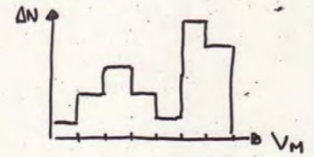
\includegraphics[scale=1]{./Immagini/Spettroscopia.png}
\caption{Esempio di spettro}
\end{center}
\end{figure}
Rimpicciolendo il numero di intervalli (in condizioni sperimentali questa suddivisione pu\`o essere spinta fino ad un certo punto) ottengo uno \textbf{spettro continuo} $\frac{dN}{dE}$.
A questo punto per conoscere il numero di particelle compreso tra due energie sar\`a sufficiente eseguire l'integrale dello spettro tra i due punti.
\subsection{Catena di lettura}
\begin{figure}[htbp]
\begin{center}
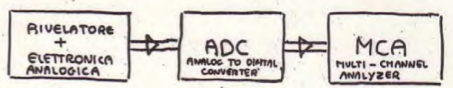
\includegraphics[scale=1]{./Immagini/CatenaDiLettura.png}
\caption{Catena di lettura}
\label{fig:CatLettura}
\end{center}
\end{figure}
La figura~\ref{fig:CatLettura} mostra la tipica catena di lettura di una spettroscopia:
\begin{enumerate}
\item Il \textbf{rivelatore}, tramite l'elettronica, produce un segnale proporzionale in tensione all'energia della particella, il segnale pu\`o essere soggetto ad un amplificazione
\item L'\textbf{Analog to Digital Converter} converte l'ampiezza del segnale ricevuto in una serie di impulsi logici, quantizzando l'ampiezza in una scala tra 1 e $2^n$ con $n$ numero di bit
\item Il \textbf{Multi Channal Analyzer} produce lo spettro, esso \`e formato da $2^n$ canali che conteggiano gli impulsi logici ricevuti, generando cos\`i lo spettro differenziale
\end{enumerate}
\section{Propriet\`a dei rivelatori}
Le caratteristiche fondamentali di un rivelatore sono:
\begin{itemize}
\item Efficienza
\item Risoluzione energetica
\item Risoluzione spaziale
\item Risoluzione temporale
\end{itemize}
\subsection{Efficienza}
L'\textbf{efficienza assoluta} di un rivelatore \`e definita come:
\begin{equation*}
\epsilon_{abs} = \frac{\text{\# di quanti rivelati}}{\text{\# di quanti emessi}}
\end{equation*}
L'efficienza assoluta dipende da diversi fattori:
\begin{enumerate}
\item Geometria del rivelatore
\item Attenuazione dal materiale
\item Efficienza di interazione
\item Efficienza di registrazione
\end{enumerate}
\subsubsection{Fattori geometrici}
Supponiamo di avere una sorgente che emette radiazione in modo isotropo, allora l'angolo solido coperto dal rivelatore risulta importante
per definire il \textbf{fattore geometrico}:
\begin{equation*}
G = \frac{\Omega}{4 \, \pi}
\end{equation*}
con $\Omega$ angolo solido coperto dal rivelatore:
\begin{equation*}
\Omega = \int_A dA \frac{\text{cos} \, \alpha }{r^2} 
\end{equation*}
con $A$ superficie del rivelatore e $\alpha$ angolo tra la normale della superficie $dA$ e la congiungente tra $dA$ e la sorgente.
\subsubsection{Attenuazione del materiale}
\`E necessario tener conto dell'effetto che il materiale ha sulla radiazione, in particolare possono esserci:
\begin{itemize}
\item Effetti di autoassorbimento della sorgente, ovvero la sorgente assorbe parte dell'energia che essa stessa emette (sorgenti spesse)
\item Effetti di assorbimento legati a materiale interposto tra sorgente e rivelatore, ad esempio dell'aria residua in casi di vuoto non ben fatto
\item Assorbimenti di energia nelle regioni di volume morto del rivelatore, ovvero regioni dove non vengono rivelati i depositi di energia da parte della radiazione.
Questo pu\`o accadere ad esempio nell'involucro del rivelatore.
\end{itemize}
\subsubsection{Efficienza di interazione}
Si definisce l'\textbf{efficienza di interazione} come:
\begin{equation*}
I = \frac{\text{\# di impulsi registrati}}{\text{\# di quanti di radiazione che incidono sul volume vivo}}
\end{equation*}
Per dei fotoni incidenti, valendo $n(x) = n_0 \, (1-\text{exp}(- \mu \cdot x))$ l'efficienza risulta:
\begin{equation*}
I = (1-\text{exp}(- \mu \cdot x))
\end{equation*}
Per le particelle cariche $I \approx 1$ in quanto \`e sufficiente una qualsiasi coppia elettrone-ione per avere una rivelazione.
\subsubsection{Efficienza di registrazione}
Viene definito come:
\begin{equation*}
R = \frac{\text{\# di impulsi registrati}}{\text{\# di interazioni}}
\end{equation*}
\subsubsection{Altre definizioni}
L'\textbf{efficienza intrinseca} indica l'efficienza del rivelatore indipendentemente dall'angolo solido coperto:
\begin{equation*}
\epsilon_{int} = \epsilon_{abs} \frac{4 \, \pi}{\Omega} = \frac{\epsilon_{abs}}{G}
\end{equation*}
L'\textbf{efficienza al picco}:
\begin{equation*}
\epsilon_{ip} = \frac{\text{\# di conteggi ad energia piena}}{\text{\# di quanti di radiazione che incidono sul rivelatore}}
\end{equation*}
\subsection{Risoluzione energetica}
Supponiamo di avere un rivelatore che emette radiazione ad energia $E$, osservando lo spettro differenziale prodotto dal MCA
si osserver\`a che esso non \`e formato da un'unica colonna, ma sar\`a formato da pi\`u colonne a distribuzione simil-gaussiana.
La \textbf{Full Width at Half Maximum} (FWHM) di questa distribuzione viene utilizzata per misurare la risoluzione energetica del dispositivo.
In particolare la FWHM pu\`o essere data in V o in eV, moltiplicando il voltaggio per il fattore di calibrazione.\\
Il deterioramento della risoluzione pu\`o essere dovuto a rumore sulla linea di base (fig.~\ref{fig:rumore}) o a fluttuazioni nella quantita di ionizzazione prodotta.
\begin{figure}[htb]
\begin{center}
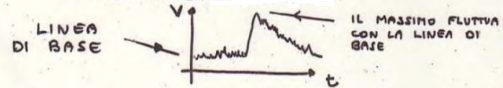
\includegraphics[scale=0.8]{./Immagini/Rumore.png}
\caption{Rumore sulla linea di base}
\label{fig:rumore}
\end{center}
\end{figure}
Altre cause del peggioramento della risoluzione possono essere trovate nella dipendenza dalla posizione della risposta del rivelatore e nella deriva temporale del fattore di calibrazione.
\subsubsection{Fluttuazioni nella generazione della carica}
Supponiamo di aver liberato $n$ portatori di carica, allora $Q = n \cdot q$ e $E = N \cdot \frac{Q}{C}$ per cui $E \propto n$,
poich\`e la ionizzazione \`e un processo statistica $n$ fluttua, le fluttuazioni di $n$ possono essere viste come un incertezza su $H$.\\
Cerchiamo di valutare quest'incertezza, il processo di ionizzazione \`e di tipo poissoniano:
\begin{equation}
P(n) = \frac{(N)^n \, e^{-N}}{n!}
\end{equation}
con $N$ numero di cariche mediamente liberate da una particella ad energia $E$ e $P(n)$ probabilit\`a di liberare $n$ cariche.
La varianza sar\`a $\sigma^2 = N$, se il numero di cariche liberate \`e sufficientemente elevato, la distribuzione pu\`o essere approssimata con una gaussiana.
Dato che $H = \frac{q \cdot n}{C}$ allora $\sigma_H = \frac{q}{C} \sigma_N = \frac{q}{C} \sqrt{N}$, per le gaussiane:
\begin{equation*}
\text{FWHM} = 2.35 \cdot \sigma_H 
\end{equation*}
mentre la risoluzione percentuale risulta:
\begin{equation*}
\frac{\text{FWHM}}{H_{max}} = \frac{2.35 \cdot \sigma_H}{H} = 2.35 \frac{1}{\sqrt{N}}
\end{equation*}
In realt\`a il processo non \`e puramente poissoniano, in quanto gli eventi non sono del tutto indipendenti, per cui vale:
\begin{equation*}
\sigma_{N}^2 = F \cdot N
\end{equation*}
con $F$ \textbf{fattore di Fano}.
\subsection{Risoluzione spaziale}
Si pu\`o ottenere della risoluzione spaziale usando rivelatori traccianti, rivelatori con elettrodi segmentati o matrici di rivelatori identici.
Si definisce \textbf{precisione spaziale} la precisione con la quale viene ricostruita la traccia lasciata dalla particella:
i punti della traccia possono essere interpolati linearmente per ottenere una traccia ben definita, la precisione viene calcolata come:
\begin{equation*}
\sigma^2 = \frac{\sum (x_{mis} - x_{interp}}{N-2}
\end{equation*}
$N-2$ \`e legato al fatto che 2 gradi di libert\`a vengono persi per via del fit lineare.\\
La \textbf{risoluzione spaziale} viene calcolata come la minima distanza tra due tracce risolte individualmente.
\subsection{Risoluzione temporale}
La \textbf{risoluzione temporale} \`e il minimo intervallo di tempo tra due eventi consecutivi che il rivelatore \`e in grado di distinguere,
corrisponde al \textbf{tempo morto} del rivelatore.
I fattori che incidono su questa caratteristica sono legati al metodo e fisica di rivelazione del dispositivo e alla strumentazione elettronica in lettura.
Se due eventi non possono essere risolti temporalmente allora pu\`o avvenire un \textit{pile-up}, questo pu\`o significare:
\begin{itemize}
\item un errato conteggio degli eventi
\item un errata valutazione dell'energia che pu\`o essere valutata come la somma delle due
\end{itemize}
\`E fondamentale riuscire a produrre delle correzioni a questo problema, prima \`e necessario distinguere tra due tipi di rivelatore: paralizzabile e non (figura~\ref{fig:tempoMorto}).
\begin{figure}[htbp]
\begin{center}
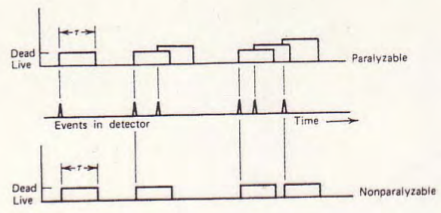
\includegraphics[scale=0.90]{./Immagini/TempoMorto.png}
\caption{Distinzione tra rivelatore paralizzabile e non.}
\label{fig:tempoMorto}
\end{center}
\end{figure}
Poniamo $n$ tasso di interazioni e $m$ tasso di rivelazioni, allora per un \textbf{rivelatore non paralizzabile} il tempo morto totale risulta
$\tau_{tot} = \tau \cdot m$, per cui il numero di interazioni reali avvenute durante questo lasso di tempo vale $n\cdot m \cdot \tau$.
Da ci\`o si deduce che in un rivelatore non paralizzabile il tasso di eventi persi vale $n \cdot (m\,\tau) = n - m$, in conclusione:
\begin{equation}\label{eq:rivnonpar}
n = \frac{m}{1-m\cdot \tau}
\end{equation}
Si osserva che nel caso di tassi $n$ molto elevati $m \approx \frac{1}{\tau}$.\\
Nel caso di un \textbf{rivelatore paralizzabile} la probabilit\`a che un intervallo sia lungo t \`e data dalla probabilit\`a che
in tale intervallo non avvenga alcun evento. 
Questa probabilit\`a \`e data dalla distribuzione di Poisson con $\lambda = n \cdot t$ e vale:
\begin{equation*}
P(0,t) dt = e^{-nt} dt
\end{equation*}
Normalizzando:
\begin{equation*}
P(0,t) dt  = n\,e^{-nt} dt
\end{equation*}
per cui la probabilit\`a che un intervallo di tempo morto sia pi\`u lungo di $\tau$ \`e:
\begin{equation*}
P(\tau) = \int_{\tau}^{\infty} P(t) \, dt = e^{-n \tau}
\end{equation*}
Per cui il tasso apparente $m$ risulta:
\begin{equation} \label{eq:rivpar}
m=n e^{-n\tau}
 \end{equation}
\subsubsection{Misura del tempo morto}
Una misura del tempo morto pu\`o essere ottenuta utilizzando una sorgente a vita media bassa, poniamo $n_b$ il tasso del fondo ambientale:
\begin{equation*}
n = n_0^{-\lambda t} + n_b
\end{equation*}
Se la sorgente ha vita media bassa allora $n_b \approx 0$:
\begin{equation*}
n = n_0^{-\lambda t}
\end{equation*}
Nel caso di un rivelatore paralizzabile da~\ref{eq:rivpar} si ha che:
\begin{equation*}
n = m \, e^{n\tau } = m \, \text{exp}(n_0 \, e^{-\lambda t})
\end{equation*}
introducendo questa espressione e applicando i logaritmi si ottiene:
\begin{equation} \label{eq:rivpartau}
\lambda t + \text{ln} m = - n_0 \tau e^{-\lambda t} + \text{ln} n_0
\end{equation}
Nel caso di un rivelatore non paralizzabile da~\ref{eq:rivnonpar} si ha:
\begin{equation} \label{eq:rivnonpartau}
m e^{\lambda t} = -n_0 \tau m + n_0
\end{equation}
Ponendo nelle equazioni~\ref{eq:rivpartau} e~\ref{eq:rivnonpartau} il lato sinistro come $y$ e $x = e^{\lambda \, t}$ 
dal coefficiente angolare \`e possibile ricavare $\tau$ e identificare il modello di rivelatore adatto.